%% ECON 282E -- Session 3, Deck B3: PyTorch, and Coding with AI
%% Budget: 16 frames (~22 minutes). Provenance: slides/SOURCES.md.
%% Ported from QM Lec. 3 section 8 (PyTorch basics) and four portable frames of
%% QM Lec. 3A (five pillars, research architect, five-step workflow, the RBC
%% worked example, validation).  The 41
%% Claude-Code product frames of 3A section 8 belong to Session 10, not here.
%% Autodiff numbers from tools/figures/s03_numbers.json, key "autodiff".

%% ECON 282E -- Foundations of Macroeconomics (UC Riverside, Fall 2026)
%% Shared Beamer preamble for every deck in slides/S01 ... slides/S10.
%%
%% Usage (a deck lives in slides/S0X/ and is compiled from that folder):
%%   %% ECON 282E -- Foundations of Macroeconomics (UC Riverside, Fall 2026)
%% Shared Beamer preamble for every deck in slides/S01 ... slides/S10.
%%
%% Usage (a deck lives in slides/S0X/ and is compiled from that folder):
%%   %% ECON 282E -- Foundations of Macroeconomics (UC Riverside, Fall 2026)
%% Shared Beamer preamble for every deck in slides/S01 ... slides/S10.
%%
%% Usage (a deck lives in slides/S0X/ and is compiled from that folder):
%%   \input{../preamble/course_preamble.tex}
%%   \decktitle{1}{A1}{Who I Am \& Why This Course}{September 24, 2026}
%%   \begin{document}
%%   \makedecktitle
%%   ...
%%
%% Adapted from Courses/AI-ECON-2026/source/shared_preamble.tex (Metropolis theme,
%% concept/caution/example/takeaway boxes, \sectiondivider). Changes for this course:
%%   * course title block (\decktitle / \makedecktitle) instead of \makebeamertitle
%%   * \zh{...} typesets Chinese (book titles) under pdflatex via CJKutf8
%%   * researchbox for the "Research in the wild" frames
%%   * section pages off; TikZ libraries and the course map loaded here
%% Build with pdflatex only (two passes); tools/build_slides.py does this for you.

\documentclass[10pt,english,aspectratio=169]{beamer}

\usepackage[T1]{fontenc}
\usepackage{textcomp}
\usepackage[utf8]{inputenc}
\usepackage{babel}
\usepackage{CJKutf8}

\usepackage{amsmath, amssymb, amsthm, graphicx}
\usepackage{booktabs, multirow, tabularx}
\usepackage{tikz}
\usetikzlibrary{positioning,arrows.meta,shapes,calc,fit,backgrounds}
\usepackage{pgfplots}
\pgfplotsset{compat=1.16}
\usepackage[most]{tcolorbox}
\tcbuselibrary{skins, breakable}
\usepackage{listings}
\usepackage{xcolor}

\lstset{
  basicstyle=\ttfamily\small,
  keywordstyle=\color{blue!80!black}\bfseries,
  commentstyle=\color{green!50!black}\itshape,
  stringstyle=\color{orange!80!black},
  backgroundcolor=\color{gray!8},
  frame=single,
  rulecolor=\color{gray!40},
  breaklines=true,
  showstringspaces=false,
  numbers=none,
}

\usetheme{metropolis}
\usefonttheme{professionalfonts}
\metroset{sectionpage=none}

\definecolor{LightGray}{RGB}{230,230,230}
\definecolor{RedTitle}{RGB}{0,0,200}
\definecolor{VeryLightGray}{RGB}{245,245,245}
\definecolor{DarkText}{RGB}{0,0,0}
\definecolor{UCRBlue}{RGB}{0,45,106}
\definecolor{UCRGold}{RGB}{241,171,0}

% Stage colours of the course arc (used by the course map and elsewhere)
\colorlet{StageTrunk}{blue!12}
\colorlet{StageBranch}{cyan!14}
\colorlet{StageMachine}{gray!18}
\colorlet{StageWall}{red!14}
\colorlet{StageTools}{orange!20}
\colorlet{StageData}{green!16}
\colorlet{StageAgents}{violet!14}

\hypersetup{bookmarks=false,breaklinks=true,pdfborder={0 0 0},colorlinks=true,
  linkcolor=DarkText,urlcolor=RedTitle}

\setbeamercolor{background canvas}{bg=white}
\setbeamercolor{title}{fg=RedTitle}
\setbeamercolor{frametitle}{bg=VeryLightGray,fg=DarkText}
\setbeamercolor{normal text}{fg=DarkText}
\setbeamercolor{alerted text}{fg=RedTitle}
\setbeamersize{text margin left=5mm, text margin right=5mm}
\addtobeamertemplate{frametitle}{}{\vspace{-0.5em}}

\setbeamertemplate{navigation symbols}{}
\setbeamertemplate{footline}{%
  \hspace{5mm}{\usebeamerfont{page number in head/foot}\color{black!45}%
  ECON 282E \,$\cdot$\, \insertshortdeck}\hfill%
  \usebeamercolor[fg]{page number in head/foot}%
  \usebeamerfont{page number in head/foot}%
  \insertframenumber\,/\,\inserttotalframenumber\kern1em\vskip2pt%
}

% ---------------------------------------------------------------------------
% Chinese text under pdflatex (book titles etc.)
\newcommand{\zh}[1]{\begin{CJK*}{UTF8}{gbsn}#1\end{CJK*}}

% ---------------------------------------------------------------------------
% Deck title block
%   \decktitle{session}{deck id}{title}{date}
\newcommand{\insertshortdeck}{}
\newcommand{\decksession}{}
\newcommand{\deckid}{}
\newcommand{\decktitletext}{}
\newcommand{\deckdate}{}
\newcommand{\decktitle}[4]{%
  \renewcommand{\decksession}{#1}%
  \renewcommand{\deckid}{#2}%
  \renewcommand{\decktitletext}{#3}%
  \renewcommand{\deckdate}{#4}%
  \renewcommand{\insertshortdeck}{Session #1 \,$\cdot$\, Deck #1.#2}%
  \title{#3}%
  \author{Zhigang Feng}%
  \date{#4}%
}
\newcommand{\makedecktitle}{%
  \begin{frame}[plain,noframenumbering]
    \begin{tikzpicture}[remember picture,overlay]
      \fill[UCRBlue] (current page.north west) rectangle ([yshift=-0.55cm]current page.north east);
      \fill[UCRGold] ([yshift=-0.55cm]current page.north west) rectangle ([yshift=-0.62cm]current page.north east);
      \node[anchor=west, text=white, font=\small\bfseries] at ([xshift=5mm,yshift=-0.275cm]current page.north west)
        {ECON 282E \,$\cdot$\, Foundations of Macroeconomics};
      \node[anchor=east, text=white, font=\small] at ([xshift=-5mm,yshift=-0.275cm]current page.north east)
        {UC Riverside \,$\cdot$\, Fall 2026};
    \end{tikzpicture}
    \vspace*{1.1cm}
    {\usebeamerfont{title}\color{black!55}\large Session \decksession\ \,$\cdot$\, Deck \decksession.\deckid\par}
    \vspace{0.25cm}
    {\usebeamerfont{title}\color{RedTitle}\LARGE\bfseries \decktitletext\par}
    \vspace{0.7cm}
    {\large Zhigang Feng\par}
    \vspace{0.15cm}
    {\color{black!65}\deckdate\par}
    \vfill
    {\footnotesize\itshape\color{black!55}Build it on paper $\;\to\;$ solve it on the machine $\;\to\;$ push it to the frontier with AI\par}
  \end{frame}}

% ---------------------------------------------------------------------------
% Section divider (plain frame, not counted)
\newcommand{\sectiondivider}[2]{%
\begin{frame}[plain,noframenumbering]
\begin{center}
\vfill
{\Large\textbf{#1}\par}
\vspace{0.35cm}
{\normalsize #2\par}
\vfill
\end{center}
\end{frame}
}

% ---------------------------------------------------------------------------
% Boxes
\newtcolorbox{conceptbox}[1][]{colback=blue!3, colframe=RedTitle!55, boxrule=0.35mm,
  arc=1mm, left=2mm, right=2mm, top=1mm, bottom=1mm, #1}
\newtcolorbox{cautionbox}[1][]{colback=red!3, colframe=red!50!black, boxrule=0.35mm,
  arc=1mm, left=2mm, right=2mm, top=1mm, bottom=1mm, #1}
\newtcolorbox{examplebox}[1][]{colback=green!3, colframe=green!45!black, boxrule=0.35mm,
  arc=1mm, left=2mm, right=2mm, top=1mm, bottom=1mm, #1}
\newtcolorbox{takeawaybox}[1][]{colback=VeryLightGray, colframe=RedTitle!55, boxrule=0.35mm,
  arc=1mm, left=2mm, right=2mm, top=1mm, bottom=1mm, #1}
\newtcolorbox{researchbox}[1][]{enhanced, colback=violet!4, colframe=violet!60!black,
  boxrule=0.35mm, arc=1mm, left=2mm, right=2mm, top=1mm, bottom=1mm,
  fonttitle=\bfseries\small, title={Research in the wild}, #1}

\newcommand{\compacttables}{\renewcommand{\arraystretch}{1.15}}
\newcommand{\src}[1]{{\tiny\color{black!55}#1}}

% ---------------------------------------------------------------------------
\input{../preamble/course_map.tex}

%%   \decktitle{1}{A1}{Who I Am \& Why This Course}{September 24, 2026}
%%   \begin{document}
%%   \makedecktitle
%%   ...
%%
%% Adapted from Courses/AI-ECON-2026/source/shared_preamble.tex (Metropolis theme,
%% concept/caution/example/takeaway boxes, \sectiondivider). Changes for this course:
%%   * course title block (\decktitle / \makedecktitle) instead of \makebeamertitle
%%   * \zh{...} typesets Chinese (book titles) under pdflatex via CJKutf8
%%   * researchbox for the "Research in the wild" frames
%%   * section pages off; TikZ libraries and the course map loaded here
%% Build with pdflatex only (two passes); tools/build_slides.py does this for you.

\documentclass[10pt,english,aspectratio=169]{beamer}

\usepackage[T1]{fontenc}
\usepackage{textcomp}
\usepackage[utf8]{inputenc}
\usepackage{babel}
\usepackage{CJKutf8}

\usepackage{amsmath, amssymb, amsthm, graphicx}
\usepackage{booktabs, multirow, tabularx}
\usepackage{tikz}
\usetikzlibrary{positioning,arrows.meta,shapes,calc,fit,backgrounds}
\usepackage{pgfplots}
\pgfplotsset{compat=1.16}
\usepackage[most]{tcolorbox}
\tcbuselibrary{skins, breakable}
\usepackage{listings}
\usepackage{xcolor}

\lstset{
  basicstyle=\ttfamily\small,
  keywordstyle=\color{blue!80!black}\bfseries,
  commentstyle=\color{green!50!black}\itshape,
  stringstyle=\color{orange!80!black},
  backgroundcolor=\color{gray!8},
  frame=single,
  rulecolor=\color{gray!40},
  breaklines=true,
  showstringspaces=false,
  numbers=none,
}

\usetheme{metropolis}
\usefonttheme{professionalfonts}
\metroset{sectionpage=none}

\definecolor{LightGray}{RGB}{230,230,230}
\definecolor{RedTitle}{RGB}{0,0,200}
\definecolor{VeryLightGray}{RGB}{245,245,245}
\definecolor{DarkText}{RGB}{0,0,0}
\definecolor{UCRBlue}{RGB}{0,45,106}
\definecolor{UCRGold}{RGB}{241,171,0}

% Stage colours of the course arc (used by the course map and elsewhere)
\colorlet{StageTrunk}{blue!12}
\colorlet{StageBranch}{cyan!14}
\colorlet{StageMachine}{gray!18}
\colorlet{StageWall}{red!14}
\colorlet{StageTools}{orange!20}
\colorlet{StageData}{green!16}
\colorlet{StageAgents}{violet!14}

\hypersetup{bookmarks=false,breaklinks=true,pdfborder={0 0 0},colorlinks=true,
  linkcolor=DarkText,urlcolor=RedTitle}

\setbeamercolor{background canvas}{bg=white}
\setbeamercolor{title}{fg=RedTitle}
\setbeamercolor{frametitle}{bg=VeryLightGray,fg=DarkText}
\setbeamercolor{normal text}{fg=DarkText}
\setbeamercolor{alerted text}{fg=RedTitle}
\setbeamersize{text margin left=5mm, text margin right=5mm}
\addtobeamertemplate{frametitle}{}{\vspace{-0.5em}}

\setbeamertemplate{navigation symbols}{}
\setbeamertemplate{footline}{%
  \hspace{5mm}{\usebeamerfont{page number in head/foot}\color{black!45}%
  ECON 282E \,$\cdot$\, \insertshortdeck}\hfill%
  \usebeamercolor[fg]{page number in head/foot}%
  \usebeamerfont{page number in head/foot}%
  \insertframenumber\,/\,\inserttotalframenumber\kern1em\vskip2pt%
}

% ---------------------------------------------------------------------------
% Chinese text under pdflatex (book titles etc.)
\newcommand{\zh}[1]{\begin{CJK*}{UTF8}{gbsn}#1\end{CJK*}}

% ---------------------------------------------------------------------------
% Deck title block
%   \decktitle{session}{deck id}{title}{date}
\newcommand{\insertshortdeck}{}
\newcommand{\decksession}{}
\newcommand{\deckid}{}
\newcommand{\decktitletext}{}
\newcommand{\deckdate}{}
\newcommand{\decktitle}[4]{%
  \renewcommand{\decksession}{#1}%
  \renewcommand{\deckid}{#2}%
  \renewcommand{\decktitletext}{#3}%
  \renewcommand{\deckdate}{#4}%
  \renewcommand{\insertshortdeck}{Session #1 \,$\cdot$\, Deck #1.#2}%
  \title{#3}%
  \author{Zhigang Feng}%
  \date{#4}%
}
\newcommand{\makedecktitle}{%
  \begin{frame}[plain,noframenumbering]
    \begin{tikzpicture}[remember picture,overlay]
      \fill[UCRBlue] (current page.north west) rectangle ([yshift=-0.55cm]current page.north east);
      \fill[UCRGold] ([yshift=-0.55cm]current page.north west) rectangle ([yshift=-0.62cm]current page.north east);
      \node[anchor=west, text=white, font=\small\bfseries] at ([xshift=5mm,yshift=-0.275cm]current page.north west)
        {ECON 282E \,$\cdot$\, Foundations of Macroeconomics};
      \node[anchor=east, text=white, font=\small] at ([xshift=-5mm,yshift=-0.275cm]current page.north east)
        {UC Riverside \,$\cdot$\, Fall 2026};
    \end{tikzpicture}
    \vspace*{1.1cm}
    {\usebeamerfont{title}\color{black!55}\large Session \decksession\ \,$\cdot$\, Deck \decksession.\deckid\par}
    \vspace{0.25cm}
    {\usebeamerfont{title}\color{RedTitle}\LARGE\bfseries \decktitletext\par}
    \vspace{0.7cm}
    {\large Zhigang Feng\par}
    \vspace{0.15cm}
    {\color{black!65}\deckdate\par}
    \vfill
    {\footnotesize\itshape\color{black!55}Build it on paper $\;\to\;$ solve it on the machine $\;\to\;$ push it to the frontier with AI\par}
  \end{frame}}

% ---------------------------------------------------------------------------
% Section divider (plain frame, not counted)
\newcommand{\sectiondivider}[2]{%
\begin{frame}[plain,noframenumbering]
\begin{center}
\vfill
{\Large\textbf{#1}\par}
\vspace{0.35cm}
{\normalsize #2\par}
\vfill
\end{center}
\end{frame}
}

% ---------------------------------------------------------------------------
% Boxes
\newtcolorbox{conceptbox}[1][]{colback=blue!3, colframe=RedTitle!55, boxrule=0.35mm,
  arc=1mm, left=2mm, right=2mm, top=1mm, bottom=1mm, #1}
\newtcolorbox{cautionbox}[1][]{colback=red!3, colframe=red!50!black, boxrule=0.35mm,
  arc=1mm, left=2mm, right=2mm, top=1mm, bottom=1mm, #1}
\newtcolorbox{examplebox}[1][]{colback=green!3, colframe=green!45!black, boxrule=0.35mm,
  arc=1mm, left=2mm, right=2mm, top=1mm, bottom=1mm, #1}
\newtcolorbox{takeawaybox}[1][]{colback=VeryLightGray, colframe=RedTitle!55, boxrule=0.35mm,
  arc=1mm, left=2mm, right=2mm, top=1mm, bottom=1mm, #1}
\newtcolorbox{researchbox}[1][]{enhanced, colback=violet!4, colframe=violet!60!black,
  boxrule=0.35mm, arc=1mm, left=2mm, right=2mm, top=1mm, bottom=1mm,
  fonttitle=\bfseries\small, title={Research in the wild}, #1}

\newcommand{\compacttables}{\renewcommand{\arraystretch}{1.15}}
\newcommand{\src}[1]{{\tiny\color{black!55}#1}}

% ---------------------------------------------------------------------------
%% Course map: the recurring "you are here" slide for ECON 282E.
%% Loaded by course_preamble.tex. Pattern follows AI-ECON-2026 lec01_map.tex, but the map
%% shows the whole ten-session course rather than one lecture.
%%
%%   \CourseMap{s}{label}   s = 1..10 highlights session s and prints "you are here: label"
%%                          (e.g. \CourseMap{1}{1.A2}); earlier sessions get a check mark.
%%   \CourseMap{0}{}        full overview, nothing highlighted.
%%
%% Note: TikZ option lists are comma-split before TeX conditionals run, so every \ifnum
%% below sits outside [...] option lists.

\newcommand{\CourseMap}[2]{%
\begin{center}
\begin{tikzpicture}[
    sess/.style={rectangle, rounded corners=2pt, draw=black!45, minimum width=1.34cm,
        minimum height=1.12cm, text width=1.26cm, align=center, inner sep=1pt},
    stage/.style={font=\tiny\bfseries, text=black!70},
]
  \foreach \i/\d/\t/\c in {%
      1/Sep 24/Intro \\ Growth/StageTrunk,
      2/Oct 1/HA $\cdot$ OLG \\ Policy/StageBranch,
      3/Oct 8/Num.\ DP \\ Python/StageMachine,
      4/Oct 15/Numerics \\ I/StageMachine,
      5/Oct 22/Numerics \\ II/StageMachine,
      6/Oct 29/The wall \\ \textbf{Midterm}/StageWall,
      7/Nov 5/ML \\ Deep nets/StageTools,
      8/Nov 12/RL \\ HA $+$ DL/StageTools,
      9/Nov 19/Text \\ LLMs/StageData,
      10/Dec 3/Agents \\ \textbf{Projects}/StageAgents} {
    \node[sess, fill=\c] (n\i) at ({1.46*(\i-1)}, 0)
      {{\scriptsize\bfseries S\i}\\[-1pt]{\tiny\color{black!60}\d}\\[1pt]{\tiny \t}};
    \ifnum\i<#1
      \node[font=\scriptsize, text=green!45!black] at ([xshift=-2.5mm,yshift=-2.2mm]n\i.north east) {$\checkmark$};
    \fi
    \ifnum\i=#1
      \draw[RedTitle, very thick, rounded corners=2pt]
        ([xshift=-0.6mm,yshift=-0.6mm]n\i.south west) rectangle ([xshift=0.6mm,yshift=0.6mm]n\i.north east);
      % keep the label inside the picture at both ends of the row
      \ifnum\i<3
        \node[font=\scriptsize\bfseries, text=RedTitle, anchor=south west] at ([yshift=1.2mm]n\i.north west)
          {$\blacktriangledown$\,you are here: #2};
      \else\ifnum\i>8
        \node[font=\scriptsize\bfseries, text=RedTitle, anchor=south east] at ([yshift=1.2mm]n\i.north east)
          {you are here: #2\,$\blacktriangledown$};
      \else
        \node[font=\scriptsize\bfseries, text=RedTitle, anchor=south] at ([yshift=1.2mm]n\i.north)
          {you are here: #2\,$\blacktriangledown$};
      \fi\fi
    \fi
  }
  % stage band under the sessions
  \foreach \a/\b/\lab/\c in {1/1/trunk/StageTrunk, 2/2/branches/StageBranch,
      3/5/the machine $\cdot$ classical methods/StageMachine, 6/6/the wall/StageWall,
      7/8/new tools/StageTools, 9/9/new data/StageData, 10/10/colleagues/StageAgents} {
    \fill[\c] ([yshift=-1.5mm]n\a.south west) rectangle ([yshift=-4.6mm]n\b.south east);
    \path ([yshift=-1.5mm]n\a.south west) -- ([yshift=-4.6mm]n\b.south east)
      node[midway, stage] {\lab};
  }
  \node[font=\footnotesize\itshape, text=black!70] at ([yshift=-9.5mm]$(n1.south)!0.5!(n10.south)$)
    {Build it on paper $\;\to\;$ solve it on the machine $\;\to\;$ push it to the frontier with AI};
\end{tikzpicture}
\end{center}
}


%%   \decktitle{1}{A1}{Who I Am \& Why This Course}{September 24, 2026}
%%   \begin{document}
%%   \makedecktitle
%%   ...
%%
%% Adapted from Courses/AI-ECON-2026/source/shared_preamble.tex (Metropolis theme,
%% concept/caution/example/takeaway boxes, \sectiondivider). Changes for this course:
%%   * course title block (\decktitle / \makedecktitle) instead of \makebeamertitle
%%   * \zh{...} typesets Chinese (book titles) under pdflatex via CJKutf8
%%   * researchbox for the "Research in the wild" frames
%%   * section pages off; TikZ libraries and the course map loaded here
%% Build with pdflatex only (two passes); tools/build_slides.py does this for you.

\documentclass[10pt,english,aspectratio=169]{beamer}

\usepackage[T1]{fontenc}
\usepackage{textcomp}
\usepackage[utf8]{inputenc}
\usepackage{babel}
\usepackage{CJKutf8}

\usepackage{amsmath, amssymb, amsthm, graphicx}
\usepackage{booktabs, multirow, tabularx}
\usepackage{tikz}
\usetikzlibrary{positioning,arrows.meta,shapes,calc,fit,backgrounds}
\usepackage{pgfplots}
\pgfplotsset{compat=1.16}
\usepackage[most]{tcolorbox}
\tcbuselibrary{skins, breakable}
\usepackage{listings}
\usepackage{xcolor}

\lstset{
  basicstyle=\ttfamily\small,
  keywordstyle=\color{blue!80!black}\bfseries,
  commentstyle=\color{green!50!black}\itshape,
  stringstyle=\color{orange!80!black},
  backgroundcolor=\color{gray!8},
  frame=single,
  rulecolor=\color{gray!40},
  breaklines=true,
  showstringspaces=false,
  numbers=none,
}

\usetheme{metropolis}
\usefonttheme{professionalfonts}
\metroset{sectionpage=none}

\definecolor{LightGray}{RGB}{230,230,230}
\definecolor{RedTitle}{RGB}{0,0,200}
\definecolor{VeryLightGray}{RGB}{245,245,245}
\definecolor{DarkText}{RGB}{0,0,0}
\definecolor{UCRBlue}{RGB}{0,45,106}
\definecolor{UCRGold}{RGB}{241,171,0}

% Stage colours of the course arc (used by the course map and elsewhere)
\colorlet{StageTrunk}{blue!12}
\colorlet{StageBranch}{cyan!14}
\colorlet{StageMachine}{gray!18}
\colorlet{StageWall}{red!14}
\colorlet{StageTools}{orange!20}
\colorlet{StageData}{green!16}
\colorlet{StageAgents}{violet!14}

\hypersetup{bookmarks=false,breaklinks=true,pdfborder={0 0 0},colorlinks=true,
  linkcolor=DarkText,urlcolor=RedTitle}

\setbeamercolor{background canvas}{bg=white}
\setbeamercolor{title}{fg=RedTitle}
\setbeamercolor{frametitle}{bg=VeryLightGray,fg=DarkText}
\setbeamercolor{normal text}{fg=DarkText}
\setbeamercolor{alerted text}{fg=RedTitle}
\setbeamersize{text margin left=5mm, text margin right=5mm}
\addtobeamertemplate{frametitle}{}{\vspace{-0.5em}}

\setbeamertemplate{navigation symbols}{}
\setbeamertemplate{footline}{%
  \hspace{5mm}{\usebeamerfont{page number in head/foot}\color{black!45}%
  ECON 282E \,$\cdot$\, \insertshortdeck}\hfill%
  \usebeamercolor[fg]{page number in head/foot}%
  \usebeamerfont{page number in head/foot}%
  \insertframenumber\,/\,\inserttotalframenumber\kern1em\vskip2pt%
}

% ---------------------------------------------------------------------------
% Chinese text under pdflatex (book titles etc.)
\newcommand{\zh}[1]{\begin{CJK*}{UTF8}{gbsn}#1\end{CJK*}}

% ---------------------------------------------------------------------------
% Deck title block
%   \decktitle{session}{deck id}{title}{date}
\newcommand{\insertshortdeck}{}
\newcommand{\decksession}{}
\newcommand{\deckid}{}
\newcommand{\decktitletext}{}
\newcommand{\deckdate}{}
\newcommand{\decktitle}[4]{%
  \renewcommand{\decksession}{#1}%
  \renewcommand{\deckid}{#2}%
  \renewcommand{\decktitletext}{#3}%
  \renewcommand{\deckdate}{#4}%
  \renewcommand{\insertshortdeck}{Session #1 \,$\cdot$\, Deck #1.#2}%
  \title{#3}%
  \author{Zhigang Feng}%
  \date{#4}%
}
\newcommand{\makedecktitle}{%
  \begin{frame}[plain,noframenumbering]
    \begin{tikzpicture}[remember picture,overlay]
      \fill[UCRBlue] (current page.north west) rectangle ([yshift=-0.55cm]current page.north east);
      \fill[UCRGold] ([yshift=-0.55cm]current page.north west) rectangle ([yshift=-0.62cm]current page.north east);
      \node[anchor=west, text=white, font=\small\bfseries] at ([xshift=5mm,yshift=-0.275cm]current page.north west)
        {ECON 282E \,$\cdot$\, Foundations of Macroeconomics};
      \node[anchor=east, text=white, font=\small] at ([xshift=-5mm,yshift=-0.275cm]current page.north east)
        {UC Riverside \,$\cdot$\, Fall 2026};
    \end{tikzpicture}
    \vspace*{1.1cm}
    {\usebeamerfont{title}\color{black!55}\large Session \decksession\ \,$\cdot$\, Deck \decksession.\deckid\par}
    \vspace{0.25cm}
    {\usebeamerfont{title}\color{RedTitle}\LARGE\bfseries \decktitletext\par}
    \vspace{0.7cm}
    {\large Zhigang Feng\par}
    \vspace{0.15cm}
    {\color{black!65}\deckdate\par}
    \vfill
    {\footnotesize\itshape\color{black!55}Build it on paper $\;\to\;$ solve it on the machine $\;\to\;$ push it to the frontier with AI\par}
  \end{frame}}

% ---------------------------------------------------------------------------
% Section divider (plain frame, not counted)
\newcommand{\sectiondivider}[2]{%
\begin{frame}[plain,noframenumbering]
\begin{center}
\vfill
{\Large\textbf{#1}\par}
\vspace{0.35cm}
{\normalsize #2\par}
\vfill
\end{center}
\end{frame}
}

% ---------------------------------------------------------------------------
% Boxes
\newtcolorbox{conceptbox}[1][]{colback=blue!3, colframe=RedTitle!55, boxrule=0.35mm,
  arc=1mm, left=2mm, right=2mm, top=1mm, bottom=1mm, #1}
\newtcolorbox{cautionbox}[1][]{colback=red!3, colframe=red!50!black, boxrule=0.35mm,
  arc=1mm, left=2mm, right=2mm, top=1mm, bottom=1mm, #1}
\newtcolorbox{examplebox}[1][]{colback=green!3, colframe=green!45!black, boxrule=0.35mm,
  arc=1mm, left=2mm, right=2mm, top=1mm, bottom=1mm, #1}
\newtcolorbox{takeawaybox}[1][]{colback=VeryLightGray, colframe=RedTitle!55, boxrule=0.35mm,
  arc=1mm, left=2mm, right=2mm, top=1mm, bottom=1mm, #1}
\newtcolorbox{researchbox}[1][]{enhanced, colback=violet!4, colframe=violet!60!black,
  boxrule=0.35mm, arc=1mm, left=2mm, right=2mm, top=1mm, bottom=1mm,
  fonttitle=\bfseries\small, title={Research in the wild}, #1}

\newcommand{\compacttables}{\renewcommand{\arraystretch}{1.15}}
\newcommand{\src}[1]{{\tiny\color{black!55}#1}}

% ---------------------------------------------------------------------------
%% Course map: the recurring "you are here" slide for ECON 282E.
%% Loaded by course_preamble.tex. Pattern follows AI-ECON-2026 lec01_map.tex, but the map
%% shows the whole ten-session course rather than one lecture.
%%
%%   \CourseMap{s}{label}   s = 1..10 highlights session s and prints "you are here: label"
%%                          (e.g. \CourseMap{1}{1.A2}); earlier sessions get a check mark.
%%   \CourseMap{0}{}        full overview, nothing highlighted.
%%
%% Note: TikZ option lists are comma-split before TeX conditionals run, so every \ifnum
%% below sits outside [...] option lists.

\newcommand{\CourseMap}[2]{%
\begin{center}
\begin{tikzpicture}[
    sess/.style={rectangle, rounded corners=2pt, draw=black!45, minimum width=1.34cm,
        minimum height=1.12cm, text width=1.26cm, align=center, inner sep=1pt},
    stage/.style={font=\tiny\bfseries, text=black!70},
]
  \foreach \i/\d/\t/\c in {%
      1/Sep 24/Intro \\ Growth/StageTrunk,
      2/Oct 1/HA $\cdot$ OLG \\ Policy/StageBranch,
      3/Oct 8/Num.\ DP \\ Python/StageMachine,
      4/Oct 15/Numerics \\ I/StageMachine,
      5/Oct 22/Numerics \\ II/StageMachine,
      6/Oct 29/The wall \\ \textbf{Midterm}/StageWall,
      7/Nov 5/ML \\ Deep nets/StageTools,
      8/Nov 12/RL \\ HA $+$ DL/StageTools,
      9/Nov 19/Text \\ LLMs/StageData,
      10/Dec 3/Agents \\ \textbf{Projects}/StageAgents} {
    \node[sess, fill=\c] (n\i) at ({1.46*(\i-1)}, 0)
      {{\scriptsize\bfseries S\i}\\[-1pt]{\tiny\color{black!60}\d}\\[1pt]{\tiny \t}};
    \ifnum\i<#1
      \node[font=\scriptsize, text=green!45!black] at ([xshift=-2.5mm,yshift=-2.2mm]n\i.north east) {$\checkmark$};
    \fi
    \ifnum\i=#1
      \draw[RedTitle, very thick, rounded corners=2pt]
        ([xshift=-0.6mm,yshift=-0.6mm]n\i.south west) rectangle ([xshift=0.6mm,yshift=0.6mm]n\i.north east);
      % keep the label inside the picture at both ends of the row
      \ifnum\i<3
        \node[font=\scriptsize\bfseries, text=RedTitle, anchor=south west] at ([yshift=1.2mm]n\i.north west)
          {$\blacktriangledown$\,you are here: #2};
      \else\ifnum\i>8
        \node[font=\scriptsize\bfseries, text=RedTitle, anchor=south east] at ([yshift=1.2mm]n\i.north east)
          {you are here: #2\,$\blacktriangledown$};
      \else
        \node[font=\scriptsize\bfseries, text=RedTitle, anchor=south] at ([yshift=1.2mm]n\i.north)
          {you are here: #2\,$\blacktriangledown$};
      \fi\fi
    \fi
  }
  % stage band under the sessions
  \foreach \a/\b/\lab/\c in {1/1/trunk/StageTrunk, 2/2/branches/StageBranch,
      3/5/the machine $\cdot$ classical methods/StageMachine, 6/6/the wall/StageWall,
      7/8/new tools/StageTools, 9/9/new data/StageData, 10/10/colleagues/StageAgents} {
    \fill[\c] ([yshift=-1.5mm]n\a.south west) rectangle ([yshift=-4.6mm]n\b.south east);
    \path ([yshift=-1.5mm]n\a.south west) -- ([yshift=-4.6mm]n\b.south east)
      node[midway, stage] {\lab};
  }
  \node[font=\footnotesize\itshape, text=black!70] at ([yshift=-9.5mm]$(n1.south)!0.5!(n10.south)$)
    {Build it on paper $\;\to\;$ solve it on the machine $\;\to\;$ push it to the frontier with AI};
\end{tikzpicture}
\end{center}
}


\graphicspath{{./figures/}}

\lstset{language=Python, basicstyle=\ttfamily\scriptsize, frame=none,
        backgroundcolor=\color{gray!8}, aboveskip=2pt, belowskip=2pt}

\decktitle{3}{B3}{PyTorch from the Ground Up, and Coding with AI}{Thursday, October 8, 2026}

\begin{document}

\makedecktitle

%=============================================================================
\begin{frame}{Where We Are}
\CourseMap{3}{3.B3}
\vspace{-1mm}
\begin{center}
\small \textbf{Block B:} \textbf{3.B1} your toolkit $\;\cdot\;$ \textbf{3.B2} from loops to arrays $\;\cdot\;$ \textbf{3.B3} PyTorch, and coding with AI $\;\cdot\;$ \textbf{3.B4} the data workflow.
\end{center}
\end{frame}

%=============================================================================
\begin{frame}{A Derivative You Cannot Get Right by Hand}
\begin{columns}[c]
\begin{column}{0.52\textwidth}
\centering
\begin{tikzpicture}
\begin{axis}[
    width=7.7cm, height=5.2cm, xmin=-16.5, xmax=-0.5, ymin=-8.4, ymax=0.9,
    xlabel={\scriptsize $\log_{10} h$}, ylabel={\scriptsize $\log_{10}$ relative error},
    tick label style={font=\scriptsize},
    axis x line*=bottom, axis y line*=left]
  \addplot[very thick, RedTitle, mark=*, mark size=1.1pt] coordinates {(-1.0,-1.808) (-2.0,-2.797) (-3.0,-3.796) (-4.0,-4.796) (-5.0,-5.796) (-6.0,-6.795) (-7.0,-7.697) (-8.0,-7.310) (-9.0,-6.276) (-10.0,-5.201) (-11.0,-5.201) (-12.0,-3.408) (-13.0,-3.408) (-14.0,-1.411) (-15.0,-1.411) (-16.0,0.000)};
  \node[font=\tiny, text=black!60, anchor=west] at (axis cs:-6.4,-1.1) {truncation};
  \node[font=\tiny, text=black!60, anchor=east] at (axis cs:-10.0,-1.1) {round-off};
  \node[font=\tiny, text=RedTitle, anchor=west] at (axis cs:-6.6,-7.35) {best: $2\times10^{-8}$};
\end{axis}
\end{tikzpicture}
\end{column}
\begin{column}{0.45\textwidth}
\small
The forward difference of $k^{\alpha}$ at $k=2$. Shrink $h$ and the approximation improves --- until round-off takes over, and at $h=10^{-16}$ the numerator underflows to zero and the answer is \textbf{100\% wrong}.
\medskip

The best you can do is about $2\times10^{-8}$, at $h\approx\sqrt{\varepsilon_{\text{mach}}}$, and you must know that in advance.
\medskip
\begin{examplebox}\footnotesize
\texttt{x.grad} $\rightarrow$ relative error \textbf{exactly 0}.
\end{examplebox}
\vspace{-1mm}
\begin{conceptbox}\footnotesize
Not a better approximation --- \emph{the same arithmetic the chain rule would give you}, done by the library.
\end{conceptbox}
\end{column}
\end{columns}
\end{frame}

%=============================================================================
\begin{frame}{What PyTorch Actually Is}
\begin{columns}[T]
\begin{column}{0.51\textwidth}
\small
Four things, and only the first two matter today:
\medskip
\begin{enumerate}\footnotesize
  \item \textbf{Tensors} --- NumPy arrays that also run on a GPU.
  \item \textbf{Autograd} --- a record of every operation, so derivatives come back exactly.
  \item \textbf{\texttt{nn.Module}} --- a class for holding parameters.
  \item \textbf{\texttt{optim}} --- gradient-descent variants.
\end{enumerate}
\medskip
It is a scientific-computing library that happens to be popular for deep learning, not the other way round.
\end{column}
\begin{column}{0.46\textwidth}
\begin{conceptbox}[title=\textbf{Why an economist needs it}]\small
Every method from here on rests on a derivative: Newton needs a Jacobian, perturbation needs high-order derivatives at the steady state, and a neural solver is trained by differentiating a residual.
\end{conceptbox}
\medskip
\begin{cautionbox}\footnotesize
And carry 3.A1's warning in: PyTorch defaults to \texttt{float32}. For anything with an accounting identity in it, set \texttt{dtype=torch.float64} explicitly.
\end{cautionbox}
\end{column}
\end{columns}
\vspace{1mm}
\src{Adapted from QM Lec.~3, ``What is PyTorch?''.}
\end{frame}

%=============================================================================
\begin{frame}[fragile]{Tensors}
\begin{columns}[c]
\begin{column}{0.48\textwidth}
\centering
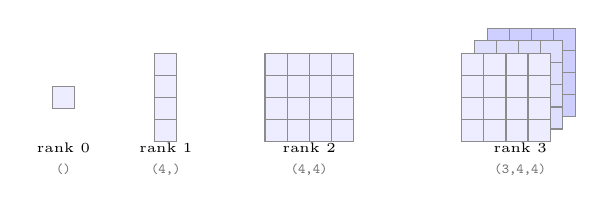
\begin{tikzpicture}[font=\tiny, cell/.style={draw=black!45, fill=blue!7, minimum size=0.28cm, inner sep=0pt}]
  % rank 0
  \node[cell] at (0,0) {};
  \node[font=\tiny, anchor=north] at (0,-0.45) {rank 0};
  \node[font=\tiny, anchor=north, text=black!55] at (0,-0.72) {\texttt{()}};
  % rank 1
  \foreach \j in {0,...,3} \node[cell] at (1.3,-\j*0.28+0.42) {};
  \node[font=\tiny, anchor=north] at (1.3,-0.45) {rank 1};
  \node[font=\tiny, anchor=north, text=black!55] at (1.3,-0.72) {\texttt{(4,)}};
  % rank 2
  \foreach \i in {0,...,3} \foreach \j in {0,...,3}
    \node[cell] at (2.7+\i*0.28,-\j*0.28+0.42) {};
  \node[font=\tiny, anchor=north] at (3.12,-0.45) {rank 2};
  \node[font=\tiny, anchor=north, text=black!55] at (3.12,-0.72) {\texttt{(4,4)}};
  % rank 3
  \foreach \k in {2,1,0}
    \foreach \i in {0,...,3} \foreach \j in {0,...,3}
      \node[cell, fill=blue!\the\numexpr7+\k*6\relax] at (5.2+\i*0.28+\k*0.16,-\j*0.28+0.42+\k*0.16) {};
  \node[font=\tiny, anchor=north] at (5.8,-0.45) {rank 3};
  \node[font=\tiny, anchor=north, text=black!55] at (5.8,-0.72) {\texttt{(3,4,4)}};
\end{tikzpicture}
\\[2mm]
\src{A scalar, a vector, a matrix and a 3-tensor are one object at different ranks. \texttt{shape} is the tuple of axis lengths.}
\end{column}
\begin{column}{0.49\textwidth}
\begin{lstlisting}
import torch

k = torch.linspace(0.05, 0.6, 200,
                   dtype=torch.float64)
k.shape, k.dtype    # (200,) float64

A = torch.zeros(200, 200)
A @ A               # matrix product
k[:, None] - k[None, :]   # broadcasting

k.numpy()                 # -> NumPy
torch.from_numpy(arr)     # <- NumPy
\end{lstlisting}
\vspace{-1mm}
\begin{examplebox}\footnotesize
Broadcasting rules are \textbf{identical} to NumPy's. Everything from 3.B2 transfers unchanged.
\end{examplebox}
\vspace{-1mm}
\begin{cautionbox}\footnotesize
\texttt{reshape} copies when it must; \texttt{view} reuses memory and refuses when it cannot. \textbf{Use \texttt{reshape}} unless you have a reason --- and either can return a \textbf{view}, which is 3.B1's copy trap one library on.
\end{cautionbox}
\end{column}
\end{columns}
\end{frame}


%=============================================================================
\begin{frame}[fragile]{Autograd: The Tape}
\begin{columns}[T]
\begin{column}{0.49\textwidth}
\begin{lstlisting}
x = torch.tensor(2.0, requires_grad=True,
                 dtype=torch.float64)
y = x ** 0.36

y.backward()      # walk the tape back
x.grad            # 0.23101666156132275

# exact: 0.36 * 2**(-0.64)
#      = 0.23101666156132275
\end{lstlisting}
\end{column}
\begin{column}{0.48\textwidth}
\small
Marking a tensor \texttt{requires\_grad} makes PyTorch \textbf{record} every operation it takes part in: nodes are tensors, edges are operations.
\medskip

\texttt{backward()} walks that graph in reverse, applying the chain rule one operation at a time. Each step is exact to machine precision, so the result is the derivative --- not an approximation of it.
\medskip
\begin{cautionbox}\footnotesize
Gradients \textbf{accumulate}. Forget \texttt{zero\_grad()} and you are descending on the sum of every gradient so far.
\end{cautionbox}
\end{column}
\end{columns}
\vspace{1mm}
\src{Adapted from QM Lec.~3, ``Autograd: Conceptual View'' and ``Autograd: Simple Example''.}
\end{frame}


%=============================================================================
\begin{frame}{Descent, in One Picture}
\begin{columns}[c]
\begin{column}{0.50\textwidth}
\centering
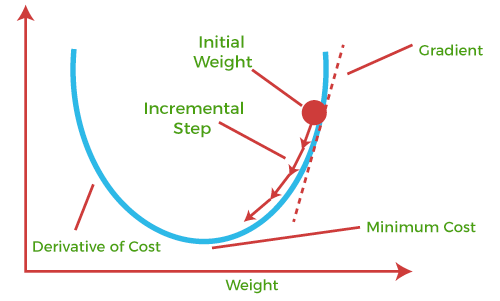
\includegraphics[width=\linewidth]{gradient_descent}\\[1mm]
\src{The loss surface, and the step $\theta\leftarrow\theta-\eta\nabla_{\theta}L$.}
\end{column}
\begin{column}{0.47\textwidth}
\small
Once derivatives are free, one algorithm covers an enormous amount of ground: write down a scalar you want small, and walk downhill.
\medskip
\begin{center}\footnotesize
\begin{tabularx}{\linewidth}{@{}>{\raggedright\arraybackslash}p{1.9cm} >{\raggedright\arraybackslash}X@{}}
\toprule
\textbf{Fit a curve} & squared prediction error \\
\textbf{Solve a model} & squared Euler residual \\
\textbf{Train a net} & either of the above \\
\bottomrule
\end{tabularx}
\end{center}
\medskip
\begin{conceptbox}\footnotesize
The middle row is the whole idea of Session 7: the residual of 3.A1 becomes a \textbf{loss}, and the policy function becomes the thing being trained.
\end{conceptbox}
\end{column}
\end{columns}
\end{frame}

%=============================================================================
\begin{frame}[fragile]{The Training Loop, Which Is Always the Same Five Lines}
\begin{columns}[T]
\begin{column}{0.53\textwidth}
\begin{lstlisting}
model = nn.Linear(4, 1)
opt   = torch.optim.Adam(model.parameters(),
                         lr=1e-3)
lossf = nn.MSELoss()

for epoch in range(n_epochs):
    opt.zero_grad()        # 1. clear
    pred = model(x)        # 2. forward
    loss = lossf(pred, y)  # 3. score
    loss.backward()        # 4. backward
    opt.step()             # 5. update
\end{lstlisting}
\end{column}
\begin{column}{0.44\textwidth}
\small
Memorise the five steps. Every PyTorch program you will read has them, in this order, and almost every bug is one of them missing.
\medskip
\begin{cautionbox}\footnotesize
\textbf{The most common bug in the world} is omitting \texttt{zero\_grad()}. It does not crash. It trains, slowly and wrongly, and the loss curve looks almost plausible.
\end{cautionbox}
\medskip
\begin{examplebox}\footnotesize
Compare it with 3.A2's loop: guess, evaluate, measure, update, repeat. Same skeleton --- only the update rule changed, from a $\max$ to a gradient step.
\end{examplebox}
\end{column}
\end{columns}
\vspace{1mm}
\src{Adapted from QM Lec.~3, ``Optimizers and Training Loop Template''.}
\end{frame}

%=============================================================================
\begin{frame}[fragile]{A Network Is a Class --- You Already Know This Pattern}
\begin{columns}[T]
\begin{column}{0.53\textwidth}
\begin{lstlisting}
class PolicyNet(nn.Module):
    def __init__(self, width=32):
        super().__init__()
        self.net = nn.Sequential(
            nn.Linear(2, width), nn.ReLU(),
            nn.Linear(width, width), nn.ReLU(),
            nn.Linear(width, 1))

    def forward(self, s):
        return self.net(s)

net = PolicyNet()
sum(p.numel() for p in net.parameters())
# 1185
\end{lstlisting}
\end{column}
\begin{column}{0.44\textwidth}
\small
Exactly the structure of \texttt{GrowthModel}: \texttt{\_\_init\_\_} sets up the state, a method supplies the behaviour. Inheriting from \texttt{nn.Module} is what makes the parameters findable by the optimiser.
\medskip
\begin{takeawaybox}\footnotesize
Read the input and output dimensions: a function of the state $(k,z)$ returning one number. That is a \textbf{policy function} --- represented by 1{,}185 numbers instead of a grid.
\end{takeawaybox}
\medskip
\begin{examplebox}\footnotesize
Which is why this matters for us: the representation no longer grows like $N^{d}$. That is the door out of the curse, and Sessions 7 and 8 walk through it.
\end{examplebox}
\end{column}
\end{columns}
\vspace{1mm}
\src{Adapted from QM Lec.~3, ``Inheritance and Why PyTorch Uses It'' and ``Reference: A Deeper MLP''.}
\end{frame}

%=============================================================================
\begin{frame}{The Five Pillars You Have to Supply}
\begin{columns}[T]
\begin{column}{0.60\textwidth}
\renewcommand{\arraystretch}{1.08}
\scriptsize
\begin{tabularx}{\linewidth}{@{}>{\raggedright\arraybackslash}p{2.1cm} >{\raggedright\arraybackslash}X c@{}}
\toprule
\textbf{Pillar} & \textbf{What you must be able to do} & \\
\midrule
Economic theory & objective, constraints, optimality conditions, equilibrium concept & S1--S2 \\
Algorithm design & turn that into an operator: Bellman or Euler, value or policy iteration & S3 \\
Numerical technique & optimization, interpolation, discretizing an AR(1), simulation & S4 \\
Advanced methods & perturbation (fast, local) against projection (global, costly), and when each is right & S5 \\
Code literacy & read a VFI loop against your design; spot a wrong index or a missing constraint & S3, labs \\
\bottomrule
\end{tabularx}
\end{column}
\begin{column}{0.37\textwidth}
\scriptsize
\begin{tabularx}{\linewidth}{@{}>{\raggedright\arraybackslash}p{1.45cm} >{\raggedright\arraybackslash}X@{}}
\toprule
\textbf{You} & \textbf{AI} \\
\midrule
the question, the model & correct syntax \\
the algorithm & the translation \\
the method & the routines \\
the accuracy criteria & the diagnostics \\
\bottomrule
\end{tabularx}
\vspace{1mm}
\begin{cautionbox}\footnotesize
The bottleneck moved: it was \emph{can you write the loop}, and it is now \textbf{can you say what the loop must satisfy, and tell whether it does}. Both are the left-hand column --- and both are how you diagnose a wrong answer.
\end{cautionbox}
\end{column}
\end{columns}
\vspace{1mm}
\src{QM Lec.~3A: the five pillar frames, ``From Foundations to AI-Assisted Coding'', ``The Core Message'' and ``What's Changing in the AI Era'' --- eight frames in one.}
\end{frame}


%=============================================================================
\begin{frame}{A Workflow That Works}
\begin{columns}[T]
\begin{column}{0.52\textwidth}
\small
\begin{enumerate}\footnotesize
  \item \textbf{Design first, separately.} Settle the model, the algorithm and the diagnostics before any code is requested.
  \item \textbf{Start at version 0} --- the case with a closed form. Ours is $\delta=1$, log utility.
  \item \textbf{Implement} one version, with the diagnostics built in from the start.
  \item \textbf{Validate} against the benchmark before adding anything.
  \item \textbf{Extend} by one feature, and re-validate.
\end{enumerate}
\end{column}
\begin{column}{0.45\textwidth}
\begin{takeawaybox}[title=\textbf{Why this order}]\small
Every step keeps a working, checkable program in your hands. When version 2 breaks, the only thing that changed is the one feature you added.
\end{takeawaybox}
\medskip
\begin{cautionbox}\footnotesize
The failure mode is asking for the full heterogeneous-agent model on the first prompt. You get 300 plausible lines, no benchmark, and no way to find out which part is wrong.
\end{cautionbox}
\end{column}
\end{columns}
\vspace{1mm}
\src{Adapted from QM Lec.~3A, ``The Five-Step Workflow'' and ``Why This Workflow Works''.}
\end{frame}


%=============================================================================
\begin{frame}{Start at Version 0, Where You Know the Answer}
\begin{columns}[T]
\begin{column}{0.49\textwidth}
\small
\textbf{Goal:} a stochastic RBC model with variable labour. \textbf{Do not start there.}
\medskip
\begin{center}\footnotesize
\begin{tabularx}{\linewidth}{@{}c >{\raggedright\arraybackslash}X >{\raggedright\arraybackslash}p{2.2cm}@{}}
\toprule
\textbf{V} & \textbf{Adds} & \textbf{Benchmark} \\
\midrule
0 & deterministic, fixed labour & closed-form steady state \\
1 & stochastic productivity & $\sigma\!\to\!0$ recovers V0 \\
2 & variable labour supply & limiting case is V1 \\
\bottomrule
\end{tabularx}
\end{center}
\medskip
\footnotesize
$k^{*}=\Big(\dfrac{\alpha\beta}{1-\beta(1-\delta)}\Big)^{\frac{1}{1-\alpha}}$ --- and at $\delta=1$ that is $(\alpha\beta)^{1/(1-\alpha)}=0.187$, \textbf{this morning's model}.
\end{column}
\begin{column}{0.48\textwidth}
\begin{conceptbox}[title=\textbf{Step 1: design, before any code}]\footnotesize
``Design a VFI algorithm for the deterministic RBC model with: (1) production $Y=K^{\alpha}$ and depreciation $\delta$; (2) Bellman equation $V(k)=\max_{k'}\ln(K^{\alpha}+(1-\delta)K-k')+\beta V(k')$; (3) grid search over $k'$.''
\end{conceptbox}
\vspace{-1mm}
\begin{examplebox}\footnotesize
Then, \emph{before} implementing: ``Can this design extend to (a) stochastic productivity with state $(k,A)$, (b) labour as a second choice? Show where each would enter.''
\end{examplebox}
\end{column}
\end{columns}
\vspace{1mm}
\src{QM Lec.~3A, ``Example 1: RBC Model'' and ``RBC: Design Algorithm First''.}
\end{frame}

%=============================================================================
\begin{frame}{Then Implement --- and Validate, Which Is Not the Same Step}
\begin{columns}[T]
\begin{column}{0.49\textwidth}
\begin{conceptbox}[title=\textbf{Step 2: implement, with diagnostics}]\footnotesize
``Implement this algorithm in Python. Include: (1) a convergence plot of $\lVert V^{n+1}-V^{n}\rVert_\infty$ against iteration; (2) the numerical $k^{*}$ against the analytical formula; (3) the policy $k'(k)$ with the 45-degree line; (4) Euler-equation residuals.''
\end{conceptbox}
\vspace{-1mm}
\footnotesize
The diagnostics are requested \textbf{in the same breath as the code}. Asking for them afterwards is how you end up with a program you cannot check.
\end{column}
\begin{column}{0.48\textwidth}
\begin{takeawaybox}[title=\textbf{Step 3: validate --- your job}]\footnotesize
\begin{itemize}
  \item Does $k'(k)$ cross the 45-degree line at the analytical $k^{*}$?
  \item Are the Euler residuals where they should be for the method? (Grid search: no. Time iteration: yes.)
  \item Do the comparative statics have the right sign --- higher $\beta$, higher $k^{*}$?
\end{itemize}
\end{takeawaybox}
\vspace{-1mm}
\begin{examplebox}\footnotesize
\textbf{Steps 4--5: extend, then re-validate.} Add the AR(1) shock; check that $\sigma=0$ reproduces Version 0 \emph{exactly}. Only then add labour.
\end{examplebox}
\end{column}
\end{columns}
\vspace{1mm}
\src{QM Lec.~3A, ``RBC: Implement and Validate''. The residual bullet is adapted: the source asks for $<10^{-8}$, which grid-search VFI cannot reach --- 3.A3 measured $10^{-1.8}$.}
\end{frame}

%=============================================================================
\begin{frame}{Validation Is the Part You Cannot Delegate}
\begin{columns}[T]
\begin{column}{0.48\textwidth}
\small
\textbf{Technical checks}
\begin{itemize}\footnotesize
  \item Does it converge, and in the expected number of iterations?
  \item Does it match the closed form?
  \item Do the Euler residuals clear $10^{-3}$ off the grid?
  \item Does the answer move when the grid or tolerance moves?
\end{itemize}
\end{column}
\begin{column}{0.49\textwidth}
\small
\textbf{Economic checks}
\begin{itemize}\footnotesize
  \item Is the policy monotone? Is $c$ increasing in wealth?
  \item Is $k^*$ near the analytical steady state?
  \item Do the comparative statics have the right \emph{sign}?
  \item Is the magnitude plausible next to data?
\end{itemize}
\end{column}
\end{columns}
\vspace{1mm}
\begin{takeawaybox}\small
\textbf{AI writes the code. You validate the economics.} An assistant can run every technical check in the left column; it has no way to notice that a 40\% capital share is absurd, and it will never tell you that the question was not worth asking.
\end{takeawaybox}
\vspace{1mm}
\src{Adapted from QM Lec.~3A, ``Validation: Your Core Responsibility''.}
\end{frame}

%=============================================================================
\begin{frame}{Takeaways}
\begin{takeawaybox}
\begin{itemize}\small
  \item Finite differences bottom out at about $2\times10^{-8}$ and then get \emph{worse} --- the round-off floor of 3.A1, in the one place it does most damage. \textbf{Automatic differentiation has no such floor}: it applies the chain rule, exactly.
  \item Tensors are NumPy arrays with a tape attached. Broadcasting, views and the copy trap all carry over unchanged. \textbf{Set \texttt{float64} yourself} --- PyTorch will not.
  \item The five-line training loop --- zero, forward, score, backward, step --- is every PyTorch program you will ever read, and \texttt{zero\_grad()} is the line people forget.
  \item A network is a class holding parameters, and a policy net is a function of the state with 1{,}185 numbers instead of a grid. That is the escape route from the curse, and the reason Block B ends here.
  \item \textbf{Specifying a problem precisely and understanding it are the same act.} Read the RBC design prompt again --- it \emph{is} 3.A1's six decisions with a benchmark attached, which is why a vague prompt is a symptom rather than a habit.
\end{itemize}
\end{takeawaybox}
\end{frame}

%=============================================================================
\begin{frame}{Bridge: The Model Gave You Numbers. So Does the World.}
\begin{columns}[T]
\begin{column}{0.52\textwidth}
\small
Everything today produced numbers out of a \emph{model}: a policy function, an iteration count, a residual. Every one was graded against a closed form, because we had one.
\medskip

Outside this benchmark you do not. What you have instead is \textbf{data} --- and a model earns its keep by reproducing moments the data actually shows. That comparison has its own workflow, and it is the last twenty minutes of the session.
\end{column}
\begin{column}{0.45\textwidth}
\begin{conceptbox}[title=\textbf{Next (3.B4)}]\small
Acquire, clean, persist, analyse, export --- and the HP filter, which is how a simulated series and a real one are made comparable.\\[1mm]
It is also the half of \textbf{Homework 1, Part B} that Block A did not give you.
\end{conceptbox}
\end{column}
\end{columns}
\end{frame}

\end{document}
